$if(has-frontmatter)$
\frontmatter
$endif$

% ---------------------------------------------------------
% Metadata from Quarto
% ---------------------------------------------------------

\newcommand{\guidelinetitle}{$title$}

$if(version)$
\newcommand{\guidelineversion}{$version$}
$else$
\newcommand{\guidelineversion}{}
$endif$

$if(date)$
\newcommand{\guidelinedate}{$date$}
$else$
\newcommand{\guidelinedate}{}
$endif$

$if(doi)$
\newcommand{\guidelinedoi}{$doi$}
$else$
\newcommand{\guidelinedoi}{}
$endif$



% ---------------------------------------------------------
% Custom title page
% ---------------------------------------------------------

\begin{titlepage}
\thispagestyle{empty}
\raggedright

% ---------------------------------------------------------
% Coverpage: Logo (upper right)
% ---------------------------------------------------------

\vspace*{-10mm}

\noindent

\makebox[\textwidth][r]{%
  
\includegraphics[
    width=0.30\textwidth
  ]{figures/coverpage/coverpage_logo.png}%
}

\par

\vspace{30mm}

% ---------------------------------------------------------
% Coverpage: Title (left aligned)
% ---------------------------------------------------------

{\fontsize{19pt}{23pt}\selectfont\bfseries\sffamily
  Magnetische Maßverkörperungen\\
  für Weg- und Winkelmesssysteme\par}

\vspace{3mm}

{\fontsize{12pt}{16pt}\selectfont\sffamily
  Terminologie, technische Darstellung, Einteilung,\\
  Messaufbau, Vermessung und Bewertung\par}

\vspace{2mm}

{\fontsize{11pt}{14pt}\selectfont\sffamily
  Version \guidelineversion\par}

\vfill

% ---------------------------------------------------------
% Coverpage: Main image (centered in text area)
% ---------------------------------------------------------

\makebox[\textwidth][c]{%
  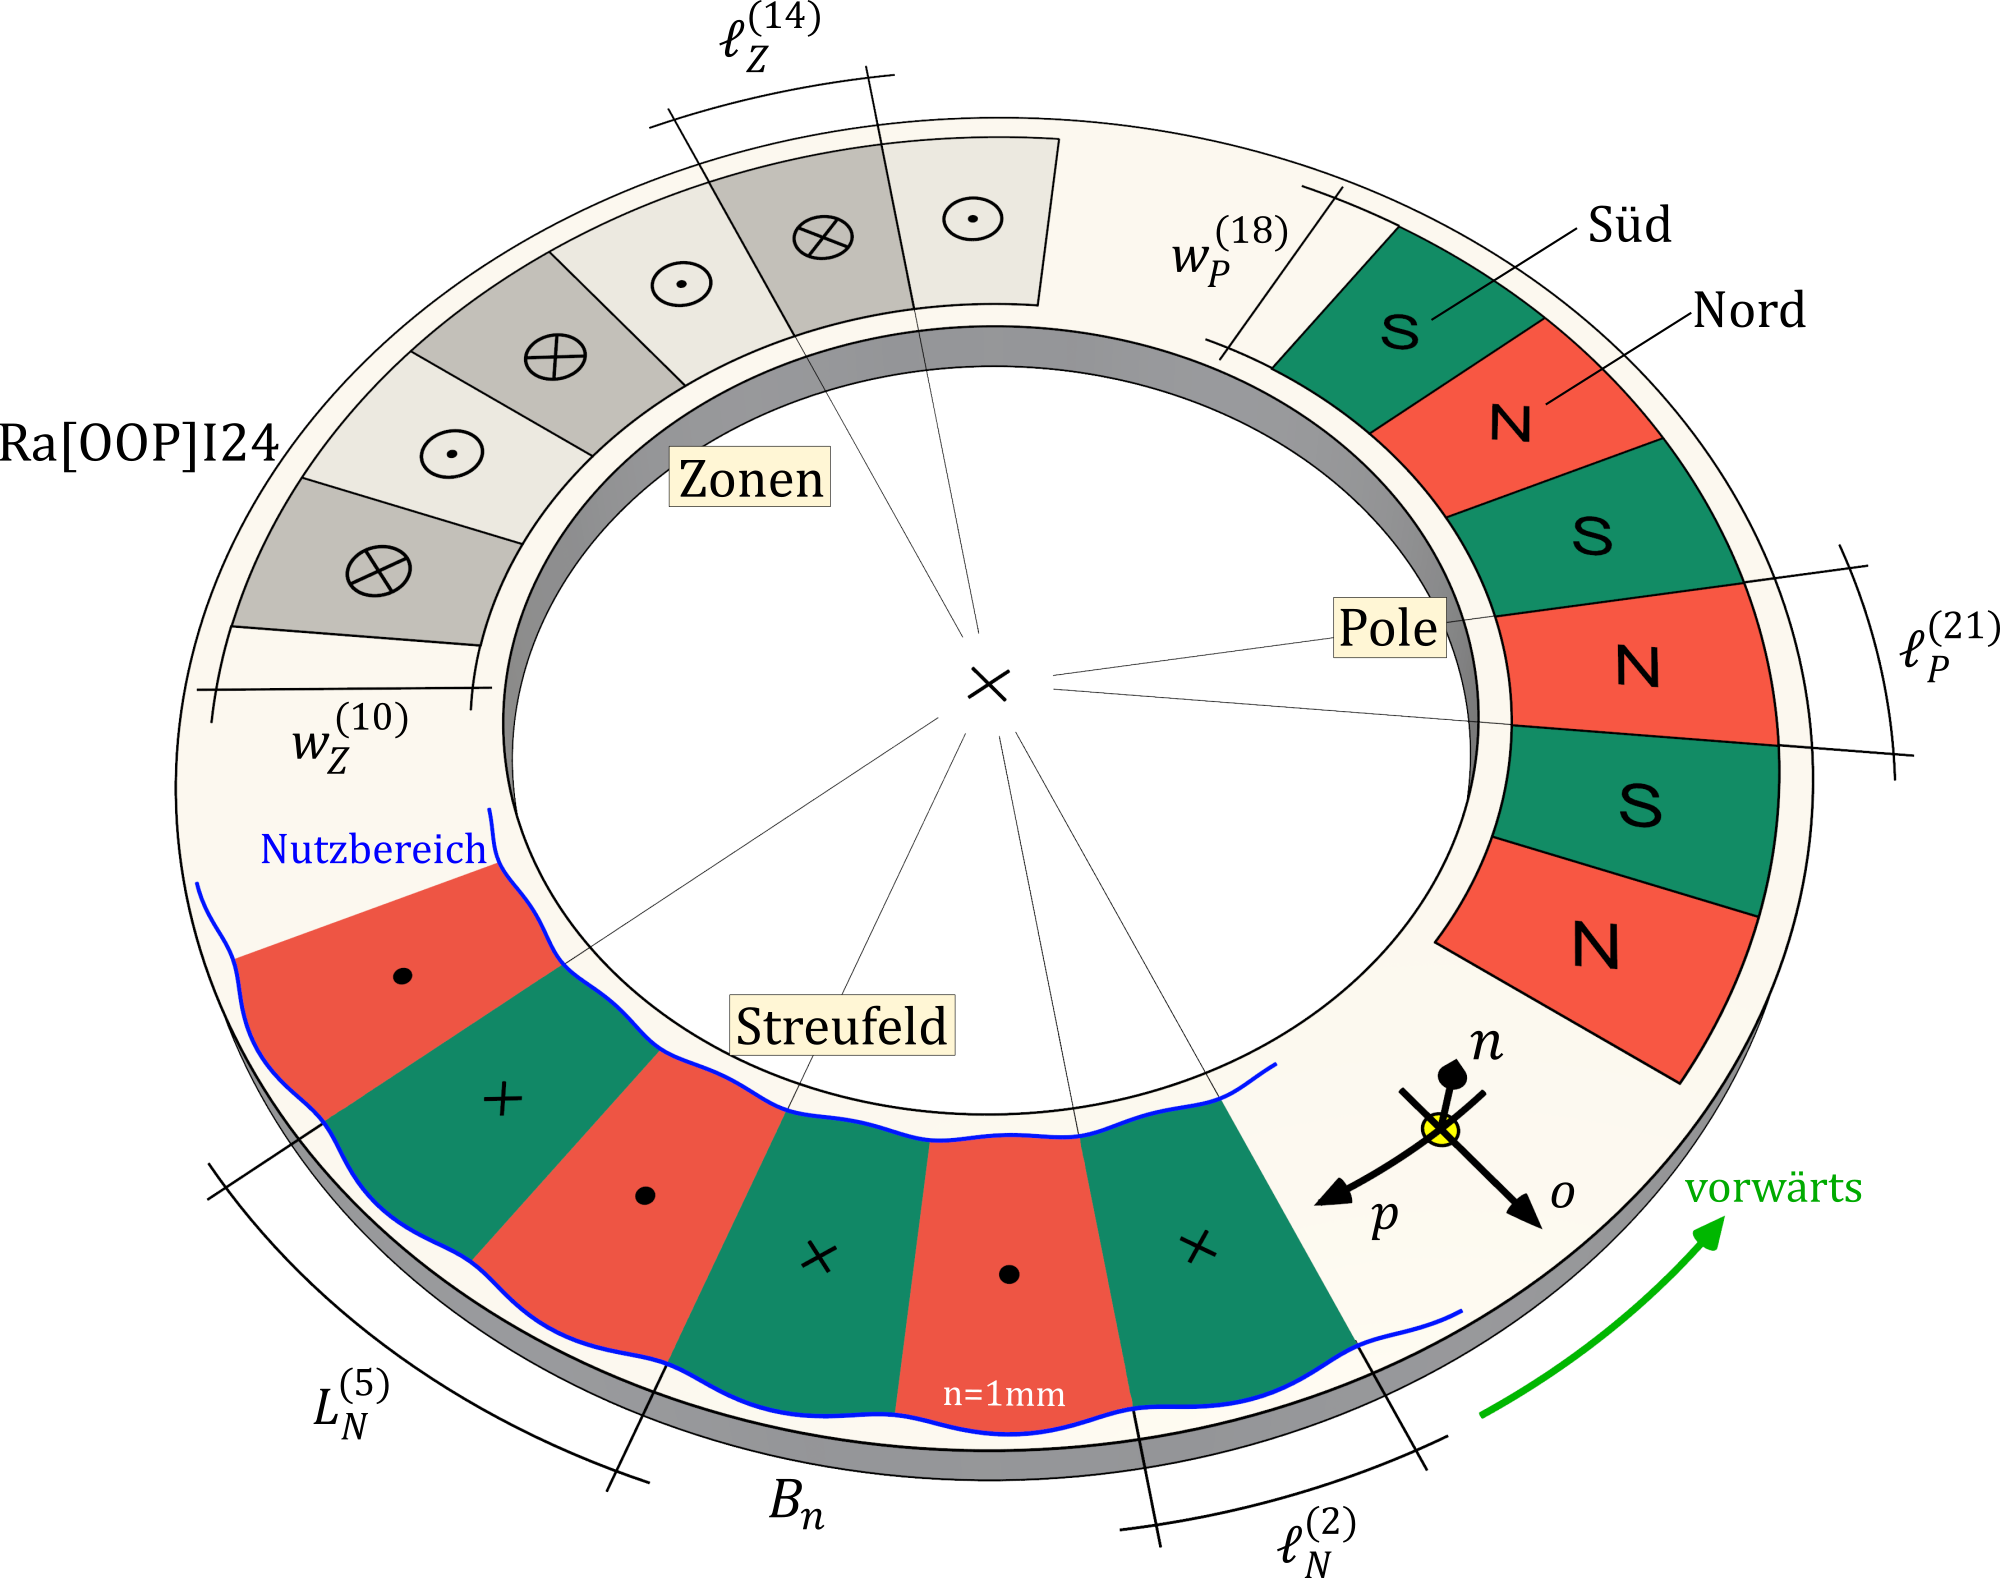
\includegraphics[
    width=0.85\textwidth,
    keepaspectratio
  ]{figures/coverpage/coverpage_image.png}%
}

\vspace*{10mm}

\end{titlepage}


% ---------------------------------------------------------
% Frontmatter: no forced blank pages
% ---------------------------------------------------------

% Im Vorwerk keine erzwungenen rechten Seiten
\KOMAoptions{open=any}

% Doppelseitenumbrüche im Vorwerk durch
% einfache Seitenumbrüche ersetzen
\let\originalcleardoublepage\cleardoublepage
\let\cleardoublepage\clearpage

% Ab dem Hauptteil normales Buchlayout wiederherstellen
\AddToHook{cmd/mainmatter/before}{%
  \let\cleardoublepage\originalcleardoublepage
  \KOMAoptions{open=right}%
}


% ---------------------------------------------------------
% Impressum
% ---------------------------------------------------------

\thispagestyle{empty}

\small

\textbf{\guidelinetitle}

\vspace{1.0cm}

\textbf{Version}: \guidelineversion

\textbf{Publikationsdatum}: \guidelinedate

\textbf{DOI}: \guidelinedoi

\vspace{1.0cm}

\textbf{Autoren}: Michael Ortner, Rolf Slatter

\textbf{Herausgeber}: INNOMAG e. V., Ruhe Almend 8, 67655 Kaiserslautern

\vspace{1.0cm}

Dieses Werk ist unter der Creative-Commons-Lizenz Namensnennung 4.0 International (CC BY 4.0) lizenziert. Ausgenommen sind Inhalte Dritter, sofern diese nicht ausdrücklich anders gekennzeichnet sind.

Das Werk darf vervielfältigt, verbreitet, bearbeitet und für beliebige Zwecke, einschließlich kommerzieller Zwecke, verwendet werden, sofern eine angemessene Namensnennung erfolgt, auf die Lizenz verwiesen wird und Änderungen kenntlich gemacht werden.

\normalsize

\clearpage

% ---------------------------------------------------------
% One intentionally blank page
% ---------------------------------------------------------

\thispagestyle{empty}
\null
\clearpage
